\documentclass[12pt, twoside]{article}
\usepackage[letterpaper, margin=1in, headsep=0.5in]{geometry}
\usepackage[english]{babel}
\usepackage[utf8]{inputenc}
\usepackage{amsmath}
\usepackage{amsfonts}
\usepackage{amssymb}
\usepackage{tikz}
\usetikzlibrary{quotes, angles}
\usepackage{graphicx}
\usepackage{enumitem}
\usepackage{multicol}

\newif\ifmeta
\metatrue %print standards and topics tags

\title{Regents Geometry}
\author{Chris Huson}
\date{September 2020}

\usepackage{fancyhdr}
\pagestyle{fancy}
\fancyhf{}
\renewcommand{\headrulewidth}{0pt} % disable the underline of the header
\raggedbottom


\fancyhead[LE]{\thepage}
\fancyhead[RO]{\thepage \\ Name: \hspace{4cm} \,\\}
\fancyhead[LO]{BECA / Dr. Huson / Geometry 09-Congruence-transformations\\* pset ID: 147}

\begin{document}

\subsubsection*{9-1DN-Correspondence}
\begin{enumerate}
\item Translate $\triangle ABC$ by $(x,y) \rightarrow (x+3, y-5)$. Label the image $\triangle A'B'C'$.
  \begin{center}
      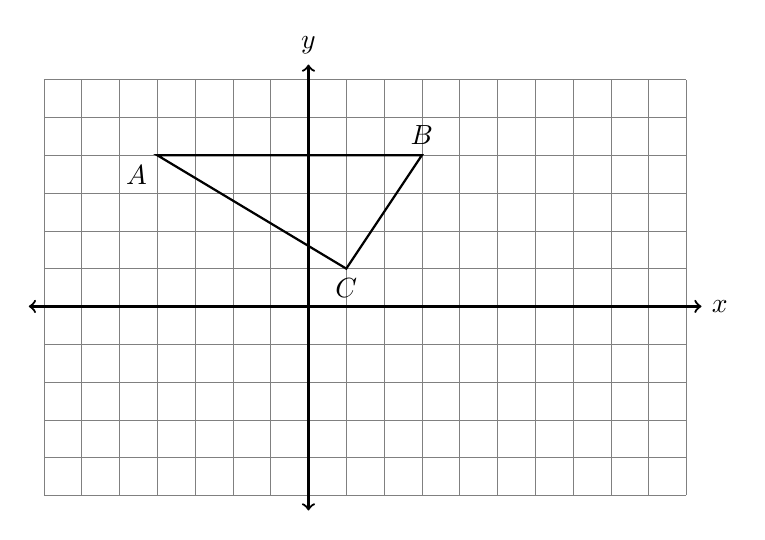
\begin{tikzpicture}[scale=.48]
      \draw [help lines] (-7,-5) grid (10,6);
      \draw [thick, <->] (-7.4,0) -- (10.4,0) node [right] {$x$};
      \draw [thick, <->] (0,-5.4)--(0,6.4) node [above] {$y$};  
      \draw [thick]
        (-4,4) node[below left] {$A$}--
        (3,4) node[above] {$B$}--
        (1,1) node[below] {$C$}--cycle;  
    \end{tikzpicture}
  \end{center}

\item What transformation maps $\triangle ABC$ onto $\triangle DEC$, shown below? Fully specify the transformation. Complete the table of mappings to  corresponding objects.  \vspace{0.5cm}
    \begin{multicols}{2}
      \begin{enumerate}
        \item $A \rightarrow$ \rule{2cm}{0.15mm}
        \item $B \rightarrow$ \rule{2cm}{0.15mm}
        \item $C \rightarrow$ \rule{2cm}{0.15mm}
        \item $\angle ACB \cong$ \rule{2cm}{0.15mm}
        \item \rule{2cm}{0.15mm} $\cong \overline {DE}$
      \end{enumerate}
      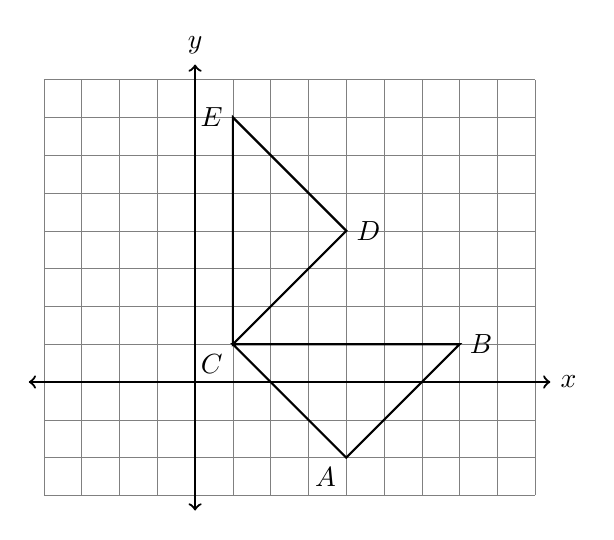
\begin{tikzpicture}[scale=.48]
        \draw [help lines] (-4,-3) grid (9,8);
        \draw [thick, <->] (-4.4,0) -- (9.4,0) node [right] {$x$};
        \draw [thick, <->] (0,-3.4)--(0,8.4) node [above] {$y$};  
        \draw [thick]
        (4,-2) node[below left] {$A$}--
        (7,1) node[right] {$B$}--
        (1,1) node[below left] {$C$}--cycle;  
        \draw [thick]
        (4,4) node[right] {$D$}--
        (1,7) node[left] {$E$}--
        (1,1) --cycle; 
      \end{tikzpicture}
    \end{multicols}
  
\item Reflect $\triangle TRS$ across the $y$-axis, labeling the image $\triangle T'R'S'$. Check those properties that are maintained by reflection. \vspace{0.5cm}
  \begin{multicols}{2}
    \begin{itemize}
      \item[$\square$] Length
      \item[$\square$] Angle measures
      \item[$\square$] Orientation
      \item[$\square$] Parallel relationships
      \item[$\square$] Area
    \end{itemize}
    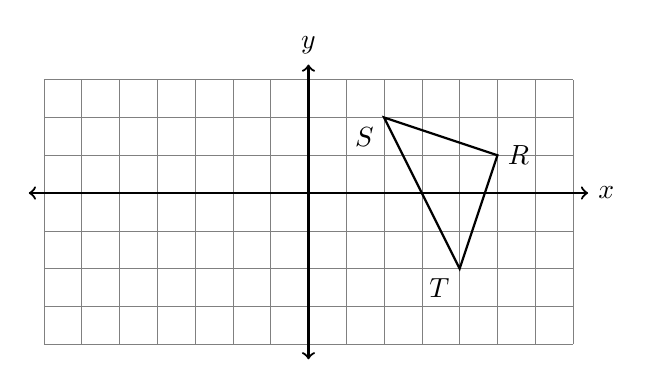
\begin{tikzpicture}[scale=.48]
      \draw [help lines] (-7,-4) grid (7,3);
      \draw [thick, <->] (-7.4,0) -- (7.4,0) node [right] {$x$};
      \draw [thick, <->] (0,-4.4)--(0,3.4) node [above] {$y$};  
      \draw [thick]
      (4,-2) node[below left] {$T$}--
      (5,1) node[right] {$R$}--
      (2,2) node[below left] {$S$}--cycle;
    \end{tikzpicture}
  \end{multicols}

\newpage
\item A translation maps triangle $PQR$ onto triangle $STU$. \vspace{0.5cm}
    \begin{multicols}{2}
      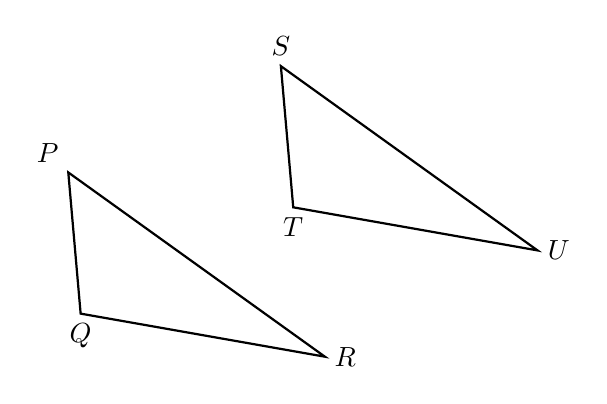
\begin{tikzpicture}[scale=0.9]
        \coordinate [label=above left:$P$](A) at (95:2);
        \coordinate [label=below:$Q$](B) at (0, 0);
        \coordinate [label=right:$R$](C) at (-10:3.5);
        \draw [thick] (A)--(B)--(C)--cycle;
        \draw [thick, xshift=3cm, yshift=1.5cm] (95:2) node[above]{$S$}--
        (0,0) node[below]{$T$}--
        (-10:3.5) node[right]{$U$}--cycle;
      \end{tikzpicture}\\
      Write each corresponding object.
      \begin{enumerate}
        \item $Q \rightarrow$ \rule{2cm}{0.15mm}
        \item $\angle QRP \cong$ \rule{2cm}{0.15mm}
        \item \rule{2cm}{0.15mm} $\cong \overline {ST}$
        \item Justify $\triangle PQR \cong \triangle STU$. Use the words ``rigid motion".
      \end{enumerate}
    \end{multicols}  \vspace{2cm}

\item Check those transformations that are rigid motions.
    \begin{itemize}
      \item[$\square$] Dilation
      \item[$\square$] Translation
      \item[$\square$] Reflection
      \item[$\square$] Rotation
      \item[$\square$] An isometry
      \item[$\square$] Horizontal stretch
    \end{itemize}

\item A rigid motion maps $\triangle DEF$ onto $\triangle LMN$. Fill in the blanks. \vspace{0.5cm}
  \begin{multicols}{2}
    The following is given:\\*[0.5cm]
    $DE=10$ \\
    $m\angle E = 40^\circ$ \\
    $m\angle F = 110^\circ$ \\[0.5cm]
    \columnbreak
    \begin{enumerate}
      \item $D \rightarrow$ \rule{2cm}{0.15mm}
      \item $LM =$ \rule{2cm}{0.15mm}
      \item $m\angle M =$ \rule{2cm}{0.15mm}
      \item $\overline{LM} \cong$ \rule{2cm}{0.15mm}
    \end{enumerate}
  \end{multicols} 

\item Given $\triangle JKL \sim \triangle MNO$. $m\angle K = 40^\circ$ and $m\angle M = 100^\circ$.\\
    Find the measure of $\angle J$. \vspace{3cm}

\end{enumerate}
\end{document}